\documentclass[shortpaper]{clv3}  %for single-spaced version
%\documentclass[manuscript]{clv3} %for double-spaced version

\usepackage[utf8]{inputenc}
\usepackage{amsmath}
\usepackage{graphicx}
\usepackage{algorithm}

\usepackage{algorithmicx}
\usepackage{algpseudocode}
\usepackage{amssymb}
\usepackage{pifont}
\usepackage{todonotes}
\usepackage{url}
\usepackage{array,multirow,graphicx}
\usepackage{rotating}
\usepackage{times}
\usepackage{latexsym}
\usepackage{arydshln}
\usepackage{enumitem}
\setlist{nolistsep} % needs enumitem

\issue{43}{3}{2017}

\title{Representation of linguistic form and function in recurrent neural networks}
\runningtitle{Representation of linguistic form and function in recurrent neural networks}

\author{Ákos Kádár \thanks{Tilburg Center for Cognition and Communication,
Tilburg University, 5000 LE Tilburg, The Netherlands, 
E-mail: \texttt{\{a.kadar, g.chrupala, a.alishahi\}@uvt.nl}} }  
\affil{Tilburg University}

\author{Grzegorz Chrupała \footnotemark[1]}
\affil{Tilburg University}

\author{Afra Alishahi \footnotemark[1]}
\affil{Tilburg University}

\runningauthor{Kádár, Chrupała and Alishahi}

\historydates{Submission received: 21st July, 2016 \\
Revised version received: 5th June, 2017 \\
Accepted for publication: 7th July, 2017}

\begin{document}
\maketitle


\section{Introduction}
\label{sec:intro}
Recurrent neural networks (RNNs) were introduced by
\cite{elman1990finding}
as a connectionist architecture with the
ability to model the temporal dimension. They have proved popular for
modeling language data as they learn representations of words and
larger linguistic units directly from the input data, without feature
engineering. Variations of the RNN architecture have been applied in
several NLP domains such as parsing \citep{vinyals2015grammar} and
machine translation \citep{Bahdanau2015}, as well as in computer
vision applications such as image generation \citep{gregor2015draw} and
object segmentation \citep{visin2015reseg}. RNNs are also important
components of systems integrating vision and language, e.g.\ image
\citep{karpathy2015deep} and video captioning \citep{yu2015video}.

These networks can represent variable-length linguistic expressions by
encoding them into a fixed-size low-dimensional vector. The nature and
the role of the components of these representations are not directly
interpretable as they are a complex, non-linear function of the
input. There have recently been numerous efforts to visualize deep
models such as convolutional neural networks in the domain of computer
vision, but much less so for variants of RNNs and for language
processing.

The present paper develops novel methods for uncovering abstract
linguistic knowledge encoded by the distributed representations of RNNs,
with a specific focus on analyzing the hidden activation patterns rather
than word embeddings and on the syntactic generalizations
that models learn to capture. In the current work we apply our methods
to a specific architecture trained on specific tasks, but also provide
pointers about how to generalize the proposed analysis to other settings.

As our case study we picked the {\sc Imaginet} model introduced by \label{explainimaginet}
\cite{chrupala2015learning}. It is a multi-task, multi-modal
architecture consisting of two Gated-Recurrent Unit (GRU)
\citep{cho2014properties,chung2014empirical} pathways and
a shared word embedding matrix. One of the GRUs ({\sc Visual}) is
trained to predict image vectors given image descriptions, while the other
pathway ({\sc Textual}) is a language model, trained to sequentially predict each
word in the descriptions. This particular
architecture allows a comparative analysis of the hidden activation
patterns between networks trained on two different tasks, while
keeping the training data and the word embeddings fixed. Recurrent neural
language models akin to {\sc Textual} which are trained to predict the
next symbol in a sequence are relatively well understood, and there
have been some attempts to analyze their internal states
\citep[among others]{elman1991distributed,karpathy2015visualizing}. In
constrast, {\sc Visual} maps a complete sequence of words to
a representation of a corresponding visual scene and is a less
commonly encountered, but a more interesting model from the point of
view of representing meaning conveyed via linguistic structure.
For comparison, we also consider a standard standalone language model.

We report a thorough quantitative analysis to provide a linguistic
interpretation of the networks' activation patterns. We present a
series of experiments using a novel method we call \emph{omission score}
to measure the importance of input tokens to the final prediction of models
that compute distributed representations of sentences.
Furthermore, we introduce a more global measure for estimating the
informativeness of various types of n-gram contexts for each model.
These techniques can be applied to various RNN architectures, Recursive
Neural Networks and Convolutional Neural Networks.

Our experiments show that the {\sc Visual} pathway in general
pays special attention to syntactic categories which carry semantic
content, and particularly to nouns. More surprisingly, this pathway also
learns to treat word types differently depending on their
grammatical function and their position in the sequential structure of
the sentence. In contrast, the {\sc Textual} pathway and the standalone
language model are especially sensitive to the local syntactic
characteristics of the input sentences.  Further analysis of the most
informative n-gram contexts for each model shows that while the
{\sc Visual} pathway is mostly sensitive to lexical (i.e., token n-gram)
contexts, the language models react more strongly to abstract contexts
(i.e., dependency relation n-grams) that represent syntactic constructions.

\section{Related Work}

%\subsection{Image--sentence ranking}

Image--sentence ranking is the task of retrieving the sentences that best describe an image, and vice-versa \cite{hodosh2013framing}. Most recent approaches are based learning to project image representations and sentence representations into a shared space using deep neural networks \cite[\textit{inter-alia}]{frome2013devise,socher2014grounded,vendrov2016order,faghri2017vse++}. 
%State-of-the-art approaches are now based on attention mechanisms that operate between both inputs \cite{Huang2017InstanceAwareIA,Lee_2018_ECCV}, but there is a continued interest in simpler approaches using average-pooled representations of both inputs \cite{vendrov2016order,faghri2017vse++}. 

More recently, there has been a focus on solving this task using multilingual data \cite{D17-1303,kadar2018conll} in the Multi30K dataset \cite{W16-3210}; an extension of the popular Flickr30K dataset into German, French, and Czech.
These works take a multi-view learning perspective in which 
images and their descriptions in multiple languages are different views of the
same concepts. The assumption is that common representations of multiple languages and perceptual stimuli 
can potentially exploit complementary information
between views to learn better representations. 
For example, \cite{rotman2018bridging} improves bilingual sentence representations by incorporating image information as a third view by Deep Partial Canonical Correlation Analysis.
More similar to our work 
\cite{D17-1303}, propose a convolutional-recurrent architecture with both an image--caption
and caption--caption loss to learn bilingual visually grounded representations. 
Their results were improved by the approach presented in \cite{kadar2018conll}, who also
shown the multilingual models outperform bilingual models, and that image--caption retrieval 
performance in languages with less resources can be improved with data from higher-resource
languages. We largely follow \citet{kadar2018conll}, however, our main interest lies in learning multimodal
and bilingual representations in the scenario where the images do not come from the same
data set i.e.: the data is presented is two sets of image--caption tuples rather than
image--caption--caption triples.

Taking a broader perspective, images have been used as pivots in multilingual multimodal language processing. On the word level this intuition is 
applied to visually grounded bilingual lexicon induction, which aims to learn 
cross-lingual word representations without aligned text using images as pivots
\cite{bergsma2011learning,kiela2015visual,vulic2016multi,hartmann2017limitations,hewitt2018learning}. Images have been used as pivots to learn translation models only from image--caption
data sets, without parallel text \cite{hitschler2016multimodal,nakayama2017zero,lee2017emergent,chen2018zero}.

%In this paper, we study approaches to training better image--sentence ranking models using out-of-domain datasets that do not have annotations in all of the necessary languages.

%Perceptual grounding in general and the visual modality specifically 
%can act as a  

%Rather than considering images as pivots between languages one can take the perspective
%that images and their descriptions in multiple languages are different views of the
%same concepts. Taking the this perspective of multi-view learning, 
%common representations of multiple languages and perceptual stimuli 
%can potentially exploit the complementary information
%between views to learn better representations. 



\section{Word learning model}
\label{sec:models}
Latest existing cross-situational models formulate word learning as a
translation problem, where the learner must decide which words in an
utterance correspond to which symbols (or potential referents) in the
perceptual context \cite{yu2007unified,fazly.etal.10csj}. For each new
utterance paired with a symbolic representation of the visual scene,
first the model decides which word is {\it aligned} with which symbol
based on previous associations between the two. Next, it uses the
estimated alignments to update the meaning representation associated
with each word.

We introduce a novel computational model for cross-situational word
learning from captioned images. We reformulate the problem of learning
the meaning of words as a translation problem between words and a {\it
  continuous} representation of the scene; that is, the visual
features extracted from the image. In this setting, the model learns
word representations by taking images and their descriptions one pair
at a time. To learn correspondences between English words and image
features, we borrow and adapt the translation-table estimation
component of the IBM Model 1 \cite{BrownPPM94}. The learning results
in a translation table between words and image-features, i.e.\ a list
of probabilities of image-features given a word.

\subsection{Visual input}
The features of the images are extracted by training a 16-layer
convolutional neural network (CNN) \cite{simonyan2014very} on an
object recognition task.\label{rev:cnndetail}\footnote{We used the F8k
  and F30k features available at
  \url{http://cs.stanford.edu/people/karpathy/deepimagesent/} and the
  data handling utilities from
  \url{https://github.com/karpathy/neuraltalk} for our
  experiments. The pre-trained CNN can be used through the Caffe
  framework \cite{jia2014caffe} and is available at the ModelZoo
  \url{https://github.com/BVLC/caffe/wiki/Model-Zoo}.} The network is
trained to discriminate among 1,000 different object labels on the
ImageNet dataset \cite{deng2009imagenet}. The last layer of the CNN
before the classification layer contains high level visual features of
the images, invariant to particulars such as position, orientation or
size.  We use the activation vector from this layer as a
representation of the visual scene described in the corresponding
caption. Each caption is paired with such a 4,096-dimensional vector
and used as input to a cross-situational word learner.
Figure~\ref{fig:dims} shows three sample images from the F8k
dataset most closely aligned with a particular dimension, as measured
by the cosine similarity between the image and a unit vector parallel
to the dimension axis. For example, dimension 1,000 seems to be related
to water, 2,000 to dogs or perhaps grass, and 3,000 to children.

 \begin{figure}
   \centering
   \begin{tabular}{c|lll}
     {\bf Dimension} & \multicolumn{3}{l}{\bf Top 3 images} \\\hline & & & \\
     1,000
     & 
\includegraphics[height=1.5cm]{chapters/TAL/flickr8k/2726262796_03bd63a155.jpg}
     & 
\includegraphics[height=1.5cm]{chapters/TAL/flickr8k/497122685_a51b29dc46.jpg}
     & 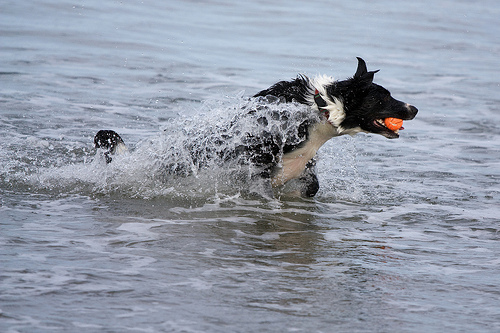
\includegraphics[height=1.5cm]{chapters/TAL/flickr8k/3515904775_f8acc5909e.jpg}
     \\
     & & & \\
     \hline
     & & & \\
     2,000
     & 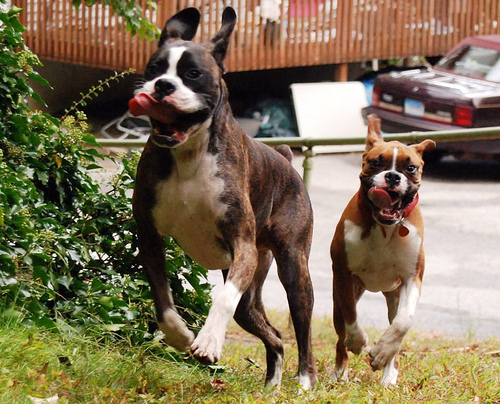
\includegraphics[height=1.5cm]{chapters/TAL/flickr8k/255741044_1102982213.jpg}
     & 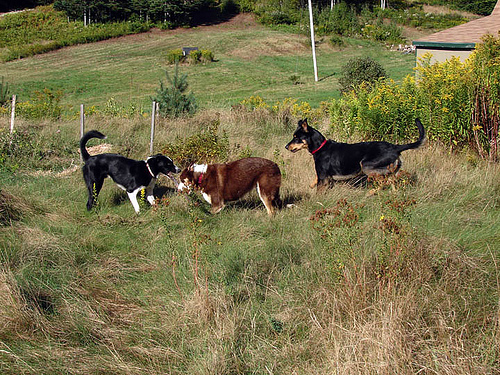
\includegraphics[height=1.5cm]{chapters/TAL/flickr8k/1388970365_162edcceb4.jpg}
     & 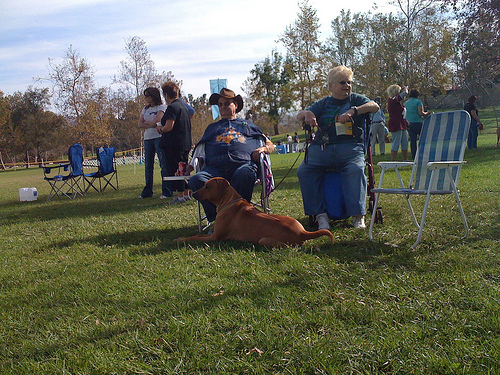
\includegraphics[height=1.5cm]{chapters/TAL/flickr8k/3053813297_7ce5f87710.jpg}
     \\
     & & & \\
     \hline
     & & & \\
     3,000
     & 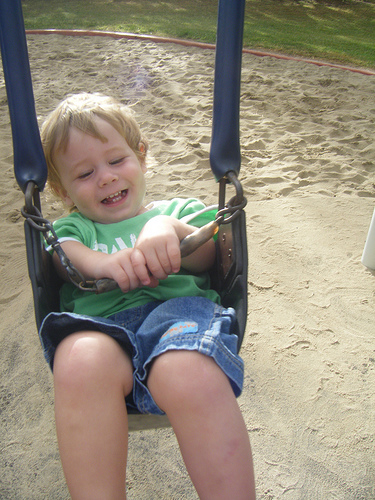
\includegraphics[height=1.5cm]{chapters/TAL/flickr8k/2362481035_a7600875d0.jpg}
     & 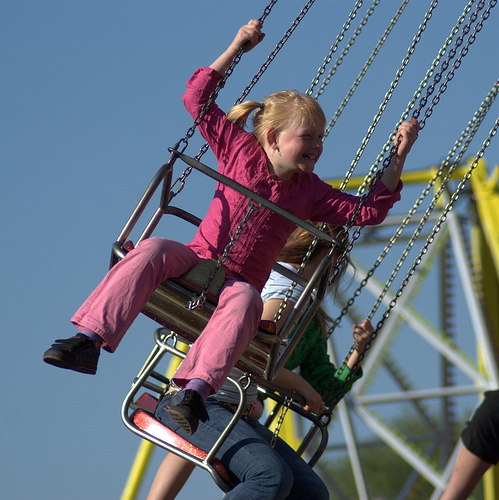
\includegraphics[height=1.5cm]{chapters/TAL/flickr8k/3504940491_94c43792ed.jpg}
     & 
\includegraphics[height=1.5cm]{chapters/TAL/flickr8k/3751594676_edfbfa0688.jpg}
     \\
     & & & \\
     \hline
   \end{tabular}
   \caption{\textit{Dimensions with three most closely aligned images from F8k.}}
   \label{fig:dims}
 \end{figure}


 \subsection{Learning algorithm}
 We adapt the IBM model 1 estimation algorithm in the following
 ways\footnote{The source code for our model is available at
   \url{https://github.com/kadarakos/IBMVisual}.}: (i) like
 \citep{fazly.etal.10csj} we run it in an online fashion, and (ii)
 instead of two sequences of words, our input consists of one sequence
 of words on one side, and a vector of real values representing the
 image on the other side. The dimensions are indexes into the visual
 feature ``vocabulary'', while the values are interpreted as weights
 of these ``vocabulary items''. In order to get an intuitive
 understanding of how the model treats the values in the feature
 vector, we could informally liken these weights to word counts.  As
 an example consider the following input with a sentence and a vector
 of 5 dimensions (i.e.\ 5 features):
\begin{itemize}
\item The blue sky
\item $(2, 0, 2, 1, 0)$
\end{itemize}
Our model treats this equivalently to the following input, with the
values of the dimensions converted to ``feature occurrences'' of each
feature $f_n$.
\begin{itemize}
\item The blue sky
\item $f_1~f_1~f_3~f_3~f_4$
\end{itemize}

The actual values in the image vectors are always non-negative, since
they come from a rectified linear (ReLu) activation. However, they can
be fractional, and thus strictly speaking cannot be literal counts. We
simply treat them as generalized, fractional feature ``counts''.  The
end result is that given the lists of words in the image descriptions
and the corresponding image vectors the model learns a probability
distribution $t(f|w)$ over feature-vector indexes $f$ for every word
$w$ in the descriptions.


\begin{algorithm}
\caption{Sentence-vector alignment model
  (\textsc{Visual})}
\label{algo:ibm-vec}
\begin{algorithmic}[1]
\State { {\bf Input:} visual feature vectors paired with sentences
  $((V_1,S_1),\ldots,(V_N,S_N))$ }
\State { {\bf Output:} translation table $t(f|w)$ }
\State { $D \leftarrow $ dimensionality of feature vectors }
\State { $\epsilon \leftarrow 1$ } \Comment {Smoothing coefficient}
\State { $a[f,w] \leftarrow 0,~ \forall f,w$ } \Comment {Initialize count tables }
\State { $a[\cdot,w] \leftarrow 0,~ \forall w$ }
\State { $t(f|w) \leftarrow \frac{1}{D}$ }
\Comment{ Translation probability $t(f|w)$ }
\For {each input pair (vector $V$, sentence $S$)}
   \For {each feature index $f \in \{1,\ldots,D\}$}
        \State { $Z_f \gets \sum_{w \in S} t(f|w)$ } \Comment { Normalization constant $Z_f$ }
        \For { each word $w$ in sentence $S$}
           \State { $c \gets \frac{1}{Z_f} \times V[f] \times
             t(f|w)$ } \Comment { Expected count $c$ }
           \State { $a[f,w] \gets a[f,w] + c$ }
           \State { $a[\cdot,w] \gets a[\cdot,w] + c$ }
           \Comment { Updates to count tables }
           \State { $t(f|w) \leftarrow \frac{a[f,w]+\epsilon}{a[\cdot,w]+\epsilon D}$ }
           \Comment { Recompute translation probabilities }
\EndFor
\EndFor
\EndFor

\end{algorithmic}
\end{algorithm}

This is our sentence-vector alignment model, \textsc{Visual}. In the
interest of cognitive plausibility, we train it using a single-pass,
online algorithm. Algorithm~\ref{algo:ibm-vec} shows the pseudo-code.
Our input is a sequence of pairs of $D$-dimensional feature vectors
and sentences, and the output is a translation table $t(f|w)$. We
maintain two count tables of expected counts $a[f,w]$ and $a[\cdot,w]$
which are used to incrementally recompute the translation
probabilities $t(f|w)$. The initial translation probabilities are
uniform \mbox{(line 7)}. In lines 12-14 the count tables are updated, based
on translation probabilities weighted by the feature value $V[f]$, and
normalized over all the words in the sentence. In line 15 the
translation table is in turn updated.

\subsection{Baseline models}
\label{sec:baseline}

To asses the quality of the meaning representations learned by our
sentence-vector alignment model \textsc{Visual}, we compare its
performance in a set of tasks to the following baselines:
\begin{itemize}
  \item \textsc{Monoling:} instead of aligning each sentence with its
    corresponding visual vector, this variation aligns two copies of
    each sentence with each other, and thus learns word
    representations based on word-word co-occurrences\footnote{This
      model does not estimate probabilities of translation of a word
      to itself, that is probabilities of the form $t(w|w)$.}.
  \item \textsc{Word2Vec:} for comparison we also report results with the skip-gram embedding model, also known as \textsc{word2vec} which builds word
    representations based on word-word co-occurrences as well
    \cite{mikolov2013efficient,mikolov2013distributed}. \textsc{Word2vec}
    learns a vector representation (embedding) of a word which
    maximizes performance on predicting words in a small window around
    it.
\end{itemize}

\section{Experiments}
\label{sec:experiments}


\subsection{Image datasets}
\label{sec:dataset}
We use image-caption datasets for our experiments.
F8k \citep{rashtchian2010collecting} consists of 8000 images and five
captions for each image. F30k \citep{young2014image} extends the F8k and contains 31,783 images
with five captions each summing up to 158,915 sentences. For both data
sets we use the splits from \cite{karpathy2014deep}, leaving out 1000
images for validation and 1000 for testing from each
set. Table~\ref{tab:flickr} summarizes the statistics of the Flickr
image-caption datasets.



\begin{table}[h]
\centering
\begin{tabular}{l|r|r}
                    & F8k    & F30k   \\ \hline
Train images        & 6,000       & 29,780  \\
Validation images   & 1,000       & 1,000   \\
Test images         & 1,000       & 1,000   \\
Image in total      & 8,000       & 31,780  \\
Captions per image  & 5           & 5      \\
Captions in total   & 40,000      & 158,900 \\
\end{tabular}
\caption{\textit{Flickr image caption datasets.}}
\label{tab:flickr}
\end{table}
For the Single-concept image descriptions experiments reported in
section \ref{sec:experiments-production}, we also use the ILSVRC2012
subset of ImageNet \citep{russakovsky2015imagenet}, a widely-used data set in the computer vision
community. It is an image database that annotates the WordNet noun
synset hierarchy with images. It contains 500 images per synset on
average.

\subsection{Word similarity experiments}
\label{sec:experiments-wsj}
A common evaluation task for assessing the quality of learned semantic
vectors for words is measuring word similarity. A number of
experiments have elicited human ratings on the similarity and/or
relatedness of a list of word pairs. For instance one of the data sets
we used was the SimLex999 data set, which contains similarity judgments
for 666 noun pairs (organ-liver 6.15), 222 verb pairs (occur-happen 1.38)
and \mbox{111 adjective pairs} (nice-cruel 0.67) elicited by 500 participants
recruited from \mbox{Mechanical Turk}\label{rev:similarity_example}.
These types of data sets are commonly used as
benchmarks for models of distributional semantics, where the learned
representations are expected to show a significant positive
correlation with human similarity judgments on a large number of word
pairs.


We selected a subset of the existing benchmarks according to the size
of their word pairs that overlap with our restricted vocabulary. We
ran a statistical power analysis test to estimate the minimum number
of required word pairs needed in our experiments. The projected sample
size was $N=210$ with $p=.05$, effect-size $r=.2$ and
$\mathit{power}=0.9$.  Thus some of the well-known benchmarks were
excluded due to their small sample size after we excluded words not
present in our datasets.\footnote{These include RG-65
  \citep{rubenstein1965contextual}, MC-30 \citep{miller1991contextual}
  and YP-130 \citep{yang2006verb}.}


The four standard benchmarks that contain the minimum number of word
pairs are: the full WS-353 \citep{finkelstein2001placing}, MTurk-771
\citep{radinsky2011word}, MEN \citep{bruni2014multimodal} and
SimLex999 \citep{hill2015simlex}. Note that the MTurk dataset only
contains similarity judgments for nouns. Also, a portion of the full
WordSim-353 dataset reports relatedness ratings instead of word
similarity.

\subsection{Effect of concreteness on similarity judgments}
\label{sec:effect-concrete}
The word similarity judgments provide a macro evaluation about the
overall quality of the learned word representations. For more
fine-grained analysis we turn to the dichotomy of concrete (e.g.\ {\it
  chair, car}) versus abstract (e.g.\ {\it love, sorrow}) nouns.
Evidence presented by \cite{recchia2012semantic} shows that in naming
and lexical decision tasks the early activation of abstract concepts
is facilitated by rich linguistic contexts, while physical contexts
promote the activation of concrete concepts. Based on these recent
findings, \cite{bruni2014multimodal} suggest that in case of
computational models {\it concrete} words (such as names for physical
objects and visual properties) are easier to learn from
perceptual/visual input and {\it abstract} words are mainly learned
based on their co-occurrence with other words in text.  Following
\cite{bruni2014multimodal}, but using novel methodology, we also test
this idea and examine whether more concrete words benefit more from
visual features compared with less concrete ones.

In their work \cite{bruni2014multimodal} use the automatic method from \cite{turney2011literal}
to assign concreteness values to words and split the MEN corpus in
concrete and abstract chunks. From their experiments they draw the
conclusion that visual information boosts their models' performance on
concrete nouns. However, whereas the multi-modal embeddings of
\cite{bruni2014multimodal} are trained using an unbalanced corpus of
large quantities of textual information and far poorer visual stimuli,
our visual embeddings are learned on a parallel corpus of sentences
paired with images. To our purposes, this balance in the sources of
information is critical as we aim at modeling word learning in humans.
As a consequence of this setting we rather hypothesized that solely relying on visual features would result
in better performance on more concrete words than on abstract ones and
conversely, learning language solely from textual features would lead to
higher correlations on the more abstract portion of the vocabulary.

To test this hypothesis, MEN, MTurk and Simlex999 datasets were
split in two halves based on concreteness score of the word pairs.
The "abstract" and "concrete" subclasses for each data set are obtained
by ordering the pairs according to their concreteness and then partition
the ordered tuples in halves\label{rev:partition_concreteness}.
We defined the concreteness of a word pair as the product of the
concreteness scores of the two words. The scores are taken from
the University of South Florida
Free Association Norms dataset \citep{nelsonuniversity}.
Table~\ref{tab:benchmarks} provides an overview of the benchmarks we use in this study.
Column "Concreteness" shows the average concreteness scores of all words pairs per data set,
while columns "Concrete" and "Abstract" contain the average concreteness of the concrete
and abstract halves of the word-pairs respectively.


\begin{table}[h]
\tabcolsep=0.11cm
\centering
\begin{tabular}{@{}lrrr||rrr@{}}
\hline
 & \multicolumn{3}{c}{\#Pairs} &  \multicolumn{3}{c}{Concreteness} \\
\hline
\hline
               & Total & F8k & F30k  & Full set & Concrete & Abstract \\ \hline
 WS353   & 353   & 104              & 232               & 25.09        & 35.44 & 16.22 \\
 SimLex999   & 999   & 412              & 733               & 23.86        & 35.72 & 11.99 \\
 MEN          & 3000  & 2069             & 2839              & 29.77        & 36.28 & 23.26 \\
 MTurk771    & 771   & 295              & 594               & 25.89        & 34.02 & 16.16 \\
\hline
\end{tabular}
\caption{\textit{Summary of the word-similarity benchmarks, showing the number of
word pairs in the benchmarks and the size of their overlap with the F8k
and F30k data sets. The table also reports the average concreteness of
the whole, concrete and abstract portions of the benchmarks.}}
\label{tab:benchmarks}
\end{table}
%As demonstrated in \Figure{fig:concreteness}, our hypothesis was
%confirmed only in case of the MEN benchmark.

\subsection{Word production}
\label{sec:experiments-production}
Learning multi-modal word representations gives us the advantage of
replicating real-life tasks such as naming visual entities. In this
study, we simulate a word production task as follows: given an image
from the test set, we rank all words in our vocabulary according to
their cosine similarity to the visual vector representing the
image. We evaluate these ranked lists in two different ways.

\subsubsection{Multi-word image descriptions.}
We use images from the test portion of the F8k and F30k datasets as
benchmarks. These images are each labeled with up to five captions, or
multi-word descriptions of the content of the image. To evaluate the
performance of our model in producing words for each image, we
construct the target description of an image as the union of the words
in all its captions \label{rev:stopword}
(with stop-words\footnote{Function words such as \emph{the, is, at, what, there};
we used the stop-word list from the Python library NLTK.} removed). We compare this set
with the top $N$ words in our predicted ranked word list.
As a baseline for this experiment we implemented a simple frequency baseline
\textsc{Freq}, which for every image retrieves the top $N$ most frequent words.
The second model \textsc{Cosine} uses our \textsc{Visual} word-embeddings
and ranks the words based on their cosine similarity to the given image.
The final model \textsc{Prior} implements a probabilistic interpretation of the task

\begin{equation}
\label{eq:proba}
P(w_{i}|i_{j}) \propto P(i_{j}|w_{i})\times{P(w_{i}),}
\end{equation}

where $w_{i}$ is a word from the vocabulary of the captions and
$i_{j}$ is an image from the collections of images $I$. The probability of an
image given a word is defined as

\begin{equation}
\label{eq:likelihood}
P(i_{j}|w_{i}) = \frac{\mathrm{cosine}(i_{j}, w_{i})} {\sum_{k=1}^{\left\vert{I}\right\vert} \mathrm{cosine}(i_{k}, w_{i}),}
\end{equation}

where $\mathrm{cosine}(i_{j}, w_{i})$ is the cosine between the vectorial representation of $i_{j}$
and the \textsc{Visual} word-embedding $w_{i}$. Since in any natural language corpus the distribution of word frequencies is expected to be very heavy tailed, in the model \textsc{Prior}, rather than using maximum likelihood estimation, we reduce the importance of the differences in word-frequencies and smooth the prior probability $P(w_{i})$ as described by equation \ref{eq:logmle}, where $N$ is the number of words in the vocabulary.

\begin{equation}
\label{eq:logmle}
P(w_{i}) = \frac{\mathrm{log}(\mathit{count}(w_{i}))}{\sum_{j=1}^N\mathrm{log}(\mathit{count}(w_{j}))}
\end{equation}

As a measure of performance, we report Precision at 5 (P@5) between the ranked word list and the target descriptions; i.e., proportion of correct target words among the top 5 predicted ranked words. Figure~\ref{fig:multiword-descriptors} shows an example of an image and its multi-word captions in the validation
portion of the F30k dataset.

\begin{figure}
\centering
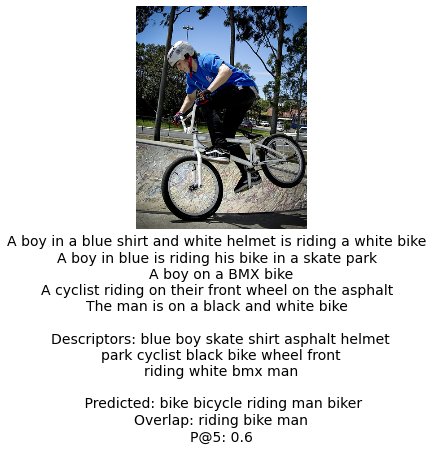
\includegraphics[scale=0.54]{chapters/TAL/bikeride}
\caption{\textit{Multiword image description example. Below the image
are the 5 captions describing the image, the union of words
that we take as targets, the top 5 predicted and the list of
correct words and the P@5 score for the given test case.}}
\label{fig:multiword-descriptors}
\end{figure}


\subsubsection{Single-concept image descriptions}
Even though we use separate portions of F8k and F30k for training and
testing, these subsets are still very similar. To test how general the
\textsc{Visual} word representations are, we use images from the ILSVRC2012
subset of ImageNet \citep{russakovsky2015imagenet} as benchmark. The major difference between these
images and the ones from F8k and F30k datasets is that labels of the
images in ImageNet are synsets from WordNet, which identify a single
concept present in the image instead of providing a natural
descriptions of its full content. Providing a quantitative evaluation
in this case is not straightforward for two main reasons. First, the
vocabulary of our model is restricted and the synsets in the ImageNet
dataset are quite varied. Second, the synset labels can be very precise,
much more so than the descriptions provided in the captions that we use
as our training data.

To attempt to solve the vocabulary mismatch problem, we use synset hypernyms
from WordNet as substitute target descriptors. If none of the lemmas
in the target synset are in the vocabulary of the model, the lemmas in
the hypernym synset are taken as new targets, until we reach the root
of the taxonomy. However, we find that in a large number of cases these hypernyms
are unrealistically general given the image. Figure \ref{fig:synset-descriptors}
illustrates these issues.

\begin{figure}
\centering
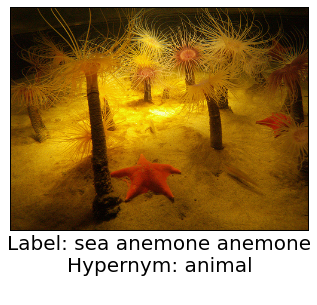
\includegraphics[scale=0.5]{chapters/TAL/starfish}
\caption{\textit{Example of the Single-concept image description task from
the validation portion of the ILSVRC2012 subset of ImageNet. The terms
"sea anemone" and "anemone" are unknown to \textsc{Visual} and "animal"
is the first word among it's hypernyms that appear in the vocabulary of F30k.}}
\label{fig:synset-descriptors}
\end{figure}

\section{Conclusions}
%\newcite{gella2017image} showed that monolingual image-sentence ranking can be improved by bilingual joint training on comparable captions using the same images. 
We learn multilingual multimodal sentence embeddings and show that multilingual joint training improves over bilingual joint training. We also demonstrate that low-resource languages can benefit from the additional data found in high-resource languages. Our experiments suggest that either translation pairs or independently-collected captions improve the performance of a multilingual model, and that the latter data setting provides further improvements through a caption--caption ranking objective. We also show that when collecting data in an additional language, it is better to collect captions for the existing images because we can exploit the caption--caption objective. Our results lead to several directions for future work. We would like to pin down the mechanism via which multilingual training contributes to improved performance for image-sentence ranking. Additionally, we only consider four languages and show the gain of multilingual over bilingual training only for the English-German language pair. In future work we will incorporate more languages from data sets such as the Chinese Flickr8K \citep{li2016adding} or Japanese COCO \citep{P16-1168}. 
%Lastly, we share all parameters across the languages; in future we will investigate other parameter sharing regimes, including character-level modeling which enables more flexible parameter sharing between languages.

%We train multilingual, multimodal sentence embeddings and through a series of image-sentence ranking experiments we show that multilingual training improves over bilingual joint training and  low-resource languages can benefit from data from high-resource languages. Our experiments suggest that both translation pairs and independently-collected captions improve performance in the multilingual setup and that the latter data setting provides more gains overall. We also find that when collecting data in an additional language, reusing the same images is more beneficial as it is possible to exploit the caption-caption (c2c) objective which enables further gains. Our results, however, lead to several new questions to be answered in future work. We would like to pin down the mechanism via which multilingual training contributes to improved performance for image-sentences ranking. Additionally we only consider four languages and show the gain of multilingual over bilingual training only for the English-German language pair. In future work we will incorporate more languages from data sets such as the Chinese Flickr8K \cite{li2016adding} or Japanese COCO \cite{P16-1168}. 
%Lastly, we share all parameters across the languages; in future we will investigate other parameter sharing regimes, including character-level modeling which enables more flexible parameter sharing between languages.

\bibliographystyle{compling}
%\starttwocolumn http://cljournal.org/commonprobs.html says we need
%this, but the template doesn't do it
\bibliography{refs}

\end{document}
